\section{Решение}

\subsection{Данные для обучения}

Стандартной практикой в области генерации данных является разделение датасетов на одноголосные (single-speaker) и многоголосные (multi-speaker), количество спикеров у которых доходит до нескольких тысяч, а количество минут чистой речи на каждого спикера -- около $20$~\cite{libritts}. Предварительные эскперименты с TalkNet показали, что для обучения эффективной многоголосной системы потребуется дополнительная контекстная информация о характере голоса, без которой сложно уловить зависимости между аудио и получить хорошее качество звучания. К примеру, в качестве эмбеддинга спикера можно использовать Global Style Token~\cite{wang2018style} или похожие эксперименты. Multi-Speaker TalkNet оставлено авторами как одно из направлений для будущей работы.

В рамках данной работы мы решили использовать данные из датасета LJSpeech~\cite{ljspeech}, который является стандартом де-факто для тестирования процесса генерации и позволяет легко сравнивать результаты с другими подходами. LJSpeech это одноголосый набор данных из 13100 отрывков семи аудиокниг документального жанра на английском языке. Размер отрывков варьируется от 1 до 10 секунд. Каждому отрывку в соответствие поставлена текстовая транскрипция с сохранением пунктуации и нормализацией чисел, денежных знаков и некоторых сокращение. Суммарная протяженность аудио -- около 24 часов.

Мы произвольно разделили набор данных на три части: $12,500$ для обучения, 300 для валидации и 300 для тестирования. Для обработки текста была использована стандартная токенизация с понижением регистра и использованием пунктуации. Таким образом мы полностью сохраняем эспрессивность текста и помогаем модели правильным образом выучить паузы, повышение тона, выделение голосом частей текста и другие особенности речи.

Как было уже сказано выше, мы не предсказывает "сырую" аудио дорожку напрямую, а используем промежуточное представление в виде мэл-спектрограмм. Такое компактное представление строится конструктивно и детерменированно из аудио с помощью оконного преобразования Фурье. Суть этой операции в последовательном применении преобразования Фурье к коротким кусочкам речевого сигнала, домноженным на некоторую оконную функцию. Результат применения оконного преобразования —- это матрица, где каждый столбец является спектром короткого участка исходного сигнала (Фигура~\ref{fig:mel-example}).

\begin{figure}[!ht]
\centering
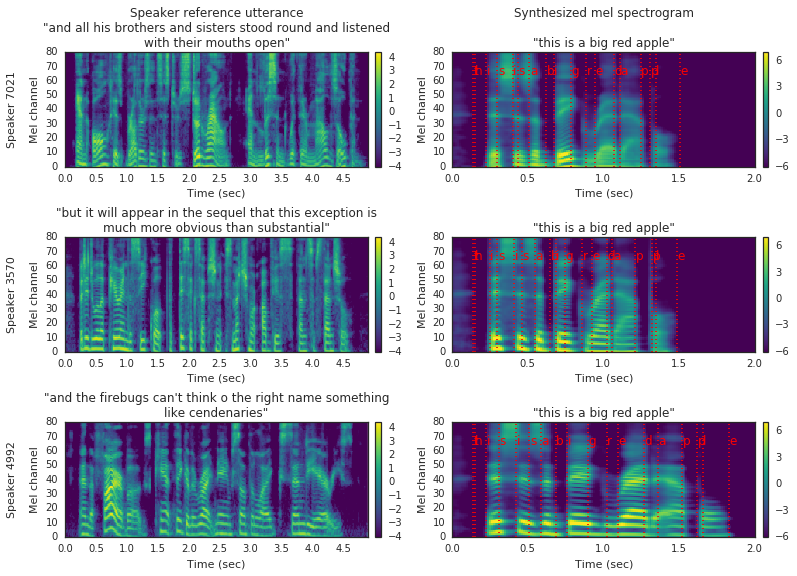
\includegraphics[width=1.0\textwidth]{images/mel-example.png}
\caption{Примеры полученных мэл-спектрограмм с выровненным текстом}
\label{fig:mel-example}
\end{figure}

Для построения мэлов мы использование библиотеку \texttt{librosa}. Мы преобразуем аудиосигналы в мэл-спектрограммы с помощью кратковременного преобразования Фурье (Short-Time Fourier Transform, STFT), используя размер окна в 50 мс с шагом в 12.5 мс, окно вида "hann" и логарифмируем результат. Более подробные характеристики преобразования: $\texttt{win\_length}=1024, \texttt{hop\_length}=256, \texttt{n\_fft}=1024, \texttt{low\_freq}=0$ и $\texttt{high\_freq}=80$.

\subsection{Обучение предсказателя длительности графем}

Как уже было сказано выше, часть TalkNet'а ответственная за предсказание длительности графен обучается отдельно. На вход такой модели подается текстовое представление токенизированное посимвольно. Далее, между каждыми соседними символами вставляется пустой (blank) символ, означающий промежуточное состояние для перевода дыхания, кратковременной паузы и итд (Рисунок~\ref{fig:durs}). Итого, общая длина входа удваивается, как и длинна выхода. Сама же модель предсказания основанна на нейронной неавторегрессионной конволюционной архитектуре QuartzNet 5x5.

Нейронная модель для предсказания длительности графемы обучалась с помощью оптимизатора Adam с $\beta_1=0.9,\beta=0.999,\epsilon=10^{-8}$, $\texttt{weight\_decay}={10}^{-6}$ и $\texttt{gradient\_norm\_clipping}=1.0$. Для $\texttt{learning\_rate}$ мы использовали cosine decay policy начиная от $10^{-3}$ до $10^{-5}$ с $\texttt{warmup}=0.02$. Для обчения использовались различные конфигурации вычислительных мощностей с 1 и 8 графическими процессорами (GPU) V100 с 16 и 32 гигабайтами видеопамяти. Мы использование батч размера 256 для одной GPU в 16GB и увеличивали $\texttt{learning\_rate}$ пропорционально увеличению мощностей. Такая конфигурация гиперпараметров позволила получить сходимость всего лишь за 200 эпох, что занимало около $1.3$ часа чистого времени на одной GPU и около $11$ минут на восьми GPU. Мы использовали обучение со смешанной точностью (mixed-precision,~\cite{micikevicius}), так как эмпирически было выявлено что такой подход позволяет получить почти двоекратное ускорение с сохранением точности.

Результаты можно увидеть на Таблице~\ref{tab:durs-results}. Как можно заметить, нам удалось получить почти 70\% точности с простой моделью, которая содердит около 2.3 миллиона весов. Более того, около 93\% предсказаний находятся на абсолютном расстоянии не более чем в 1.

\subsection{Обучение генератора мэл-спектрограмм}

Генератор мэл-спектрограм производится из символьной входной последовательности после операции расширения (expansion), в результате которой мы выравниваем длинну текста и длинну мэла по времени (Рисунок~\ref{fig:arch}). Такое выравнивание соотносит буквы с произносимыми звуками и переходами между ними, облегчая процесс генерации. В качестве длительностей графем для тренировки мы используем полученные на этапе извлечения. Таким образом, обучение генератора не требует использования предобученного предиктора длительностей и может выполняться парралельно. Сама же модель генератора основанна на нейронной неавторегрессионной конволюционной архитектуре QuartzNet 9x5.

Как видно из Таблицы~\ref{tab:durs-results}, точность предсказателя длительностей составляет около $70\%$. В то же время, количество классов находящихся на абсолютном расстоянии не более 1 - около $92\%$. Для того чтобы уменьшить несоотвествие, которое возникает на этапе вывода (inference), были применены аугментации для истинных длительностей подающихся к обоим частям модели. Такие аугментации должны отвечать некоторых заданным критериям:
\begin{enumerate}
    \item Сохранять сумму длительностей всех букв неизменной, так как она напрямую зависимт от длины мэл-спектрограммы.
    \item Быть несмещенными относительно истинных длительностей.
    \item Сила изменений для каждого символа должна быть пропорицональна длительности. Таким образом, мы будем изменять символы с большими длительностями чаще.
    \item Сила аугментации должна быть контролируема с заданным параметром.
\end{enumerate}

Одной из аументаций, удолетворяющих всем вышеперечисленным условия, может являться "биномиальная встряска" (binominal shake). Суть заключается в "обмене" длительностями соседних символов $l$ и $r$ по биномиальному распределению с заданым параметром $p$ и $n=\min(d_l, d_r)$. Каждый символа обменивается длительностями с двумя соседями, а направление обмена выбирается случайным образом с вероятностью $p=0.5$ (Рисунок~\ref{fig:aug}).

\begin{figure}[!ht]
\centering
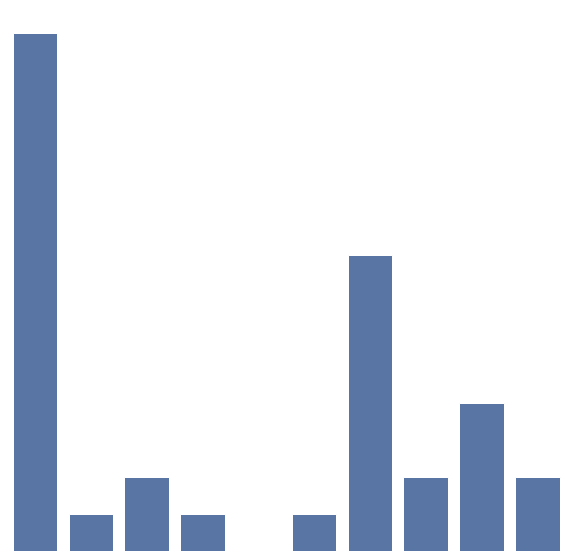
\includegraphics[width=0.49\textwidth]{images/aug/before.png}
\vrule
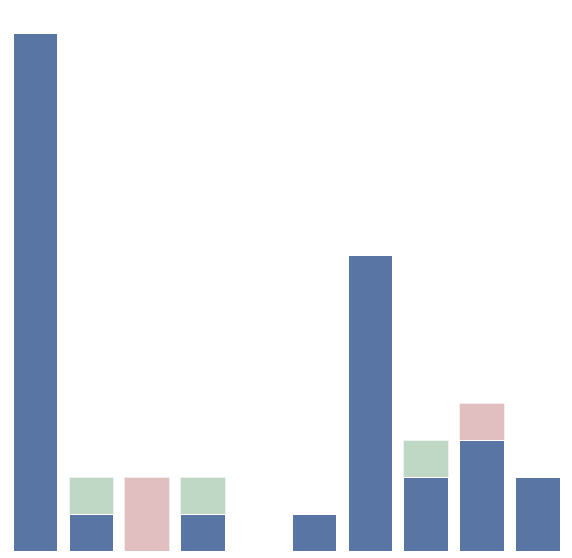
\includegraphics[width=0.49\textwidth]{images/aug/after.png}
\caption{Пример применения аугментация для длительностей графем для соседних символов. Слева - до, справа - после.}
\label{fig:aug}
\end{figure}

Опытным путем было выяснено, что аугментации помогают качеству звучания и уменьшают эффект переобучения (overfitting). Для тренировки генератора мэл-спектрограм мы применяли "биномиальную встряску" с $p=0.05$ для аугментации истинных длительностей.

Для тренировки генератора мэлов использовался тот же набор гиперпараметров, что и для предсказателя графем. Мы использование батч размера 64 для одной GPU в 16GB и увеличивали $\texttt{learning\_rate}$ пропорционально увеличению мощностей. Такая конфигурация позволила получить сходимость всего лишь за 200 эпох, что занимало около $8$ часа чистого времени на одной GPU и около $2$ часов на восьми GPU. Мы использовали обучение со смешанной точностью (mixed-precision,~\cite{micikevicius}), так как эмпирически было выявлено что такой подход позволяет получить почти двоекратное ускорение с сохранением качества.

Таким образом, процесс обучения обеих частей TalkNet'а на сервере DGX-1 может занимать всего порядка 2-ух часов. Это сравнимо меньше $2-3$ дней которые требуются модели Tacotron2~\cite{tacotron2}. Такая особенность связана прежде всего с эффектом неавторегрессионности, а также отсутствием операций основанных на механизмах внимания (attention), которые обычно занимают порядка $O(T^2)$ времени в зависимости от длины $T$.